\documentclass[12pt, titlepage]{article}

\usepackage{amsmath, mathtools}
\usepackage{amsfonts}
\usepackage{amssymb}
\usepackage{graphicx}
\usepackage{colortbl}
\usepackage{xr}
\usepackage{hyperref}
\usepackage{longtable}
\usepackage{xfrac}
\usepackage{tabularx}
\usepackage{siunitx}
\usepackage{booktabs}
\usepackage{caption}
\usepackage{multirow}
\usepackage{pdflscape}
\usepackage{afterpage}
\usepackage[table,xcdraw]{xcolor}
\hypersetup{
    colorlinks,
    citecolor=blue,
    filecolor=black,
    linkcolor=red,
    urlcolor=blue
}
\usepackage[round]{natbib}

%% Comments

\usepackage{color}

\newif\ifcomments\commentstrue %displays comments
%\newif\ifcomments\commentsfalse %so that comments do not display

\ifcomments
\newcommand{\authornote}[3]{\textcolor{#1}{[#3 ---#2]}}
\newcommand{\todo}[1]{\textcolor{red}{[TODO: #1]}}
\else
\newcommand{\authornote}[3]{}
\newcommand{\todo}[1]{}
\fi

\newcommand{\wss}[1]{\authornote{blue}{SS}{#1}} 
\newcommand{\plt}[1]{\authornote{magenta}{TPLT}{#1}} %For explanation of the template
\newcommand{\an}[1]{\authornote{cyan}{Author}{#1}}

%% Common Parts

\newcommand{\progname}{Optimal EM Placement} % PUT YOUR PROGRAM NAME HERE
\newcommand{\authname}{Hussein Saad} % AUTHOR NAMES                  

\usepackage{hyperref}
    \hypersetup{colorlinks=true, linkcolor=blue, citecolor=blue, filecolor=blue,
                urlcolor=blue, unicode=false}
    \urlstyle{same}
                                


% For easy change of table widths
\newcommand{\colZwidth}{1.0\textwidth}
\newcommand{\colAwidth}{0.13\textwidth}
\newcommand{\colBwidth}{0.82\textwidth}
\newcommand{\colCwidth}{0.1\textwidth}
\newcommand{\colDwidth}{0.05\textwidth}
\newcommand{\colEwidth}{0.8\textwidth}
\newcommand{\colFwidth}{0.17\textwidth}
\newcommand{\colGwidth}{0.5\textwidth}
\newcommand{\colHwidth}{0.28\textwidth}

\begin{document}

\title{System Verification and Validation Plan for \progname{}} 
\author{\authname}
\date{\today}
	
\maketitle

\pagenumbering{roman}

\section*{Revision History}

\begin{tabularx}{\textwidth}{p{3.5cm}p{2cm}X}
\toprule {\bf Date} & {\bf Version} & {\bf Notes}\\
\midrule
April 13, 2025 & 1.1 & Implement domain expert suggestions\\
\midrule
February 23, 2025 & 1.0 & Initial draft\\
\bottomrule
\end{tabularx}


\newpage

\tableofcontents
\newpage

\section{Symbols, Abbreviations, and Acronyms}

\renewcommand{\arraystretch}{1.2}
\begin{tabular}{l l} 
  \toprule		
  \textbf{symbol} & \textbf{description}\\
  \midrule 
  T & Test\\
  EM & Electromagnet\\
  VnV & Verification and Validation \\
  SRS & Software Requirements Specification \\
  PV & Positive value required \\
  TL & Input parameter too large \\
  \bottomrule
  \label{abbrevs}
\end{tabular}\\

\newpage

\pagenumbering{arabic}

This document provides the road-map of the verification and validation plan for Optimal EM Placement. The plan ensures the requirements and models in the SRS document are correctly implemented. It starts with introducing general information about the program in Section \ref{gen_info}, followed by a plan, and then an outline of system tests in Section \ref{sys_tests}. Finally, a description of unit tests for functional and non-functional requirements is provided in Section \ref{unit_tests}.

\section{General Information} \label{gen_info}

\subsection{Summary}
This document outlines the verification and validation plan for Optimal EM Placement, a program that calculates the optimal positions of EM actuators that yield the highest system manipulability, as defined in the \href{https://github.com/husseinsd1/optimal-em-arrangement/blob/main/docs/SRS/SRS.pdf}{SRS}. 

\subsection{Objectives}
The main purpose of this document is to define how validation will be performed for the requirements outlined in the \href{https://github.com/husseinsd1/optimal-em-arrangement/blob/main/docs/SRS/SRS.pdf}{SRS} document. The verification plan includes strategies to ensure the correct execution of system requirements testing. In particular, the VnV document devises procedures to confirm that intermediate data and computations are approximately correct, and conform to the theoretical expectations laid out in the SRS. The optimal EM positions are solved for by the \href{https://www.cvxpy.org/}{$\texttt{cvxpy}$} library --- a popular open-source convex optimization library --- which is assumed to be reliable and correct for the purposes of this project. In general, we aim to build maximum confidence in the correctness of our program. Additionally, the document outlines methods to verify that the input interface and output format are sufficiently accessible and interpretable by the intended users, as defined in the SRS. However, extensive usability verifications, beyond what is necessary for the outlined user backgrounds, is not within scope of this project.

\subsection{Challenge Level and Extras}
This project is an advanced project as it is the product of research work that will later be submitted for publication in an academic conference/journal.  

\subsection{Relevant Documentation}
The \href{https://github.com/husseinsd1/optimal-em-arrangement/blob/main/docs/ProblemStatementAndGoals/ProblemStatement.pdf}{Problem Statement} motivates the program while the \href{https://github.com/husseinsd1/optimal-em-arrangement/blob/main/docs/SRS/SRS.pdf}{SRS} provides information about the requirements of the functioning program. The MG and MIS documents contain architecture and design rationale. 

\section{Plan}
This section outlines the testing plan for the Optimal EM Placement program, starting with the team in Section \ref{team}, followed by the SRS verification plan, design verification plan, VnV verification plan, implementation verification plan, automated testing, ending with verification tools in Section~\ref{ver_tools}.

\subsection{Verification and Validation Team} \label{team}
% \begin{table}[]
%   \begin{tabular}{|c|c|c|c|}
%     \hline
%     \rowcolor[HTML]{FFC702} 
%     Name & Document & Role               & Description                                         \\ \hline
%     Hussein Saad & All      & Author             & Execution and management of VnV document and tests. \\ \hline
%     Dr. Spencer Smith & All      & Instructor         & Review all documents.                               \\ \hline
%     Uriel Cruz & All      & Domain Expert      & Review document and provide technical feedback.     \\ \hline
%     Alaap Grandhi & VnV      & Secondary Reviewer & Review the VnV plan and suggest improvements.       \\ \hline
%   \end{tabular}
% \end{table}
\begin{center}
  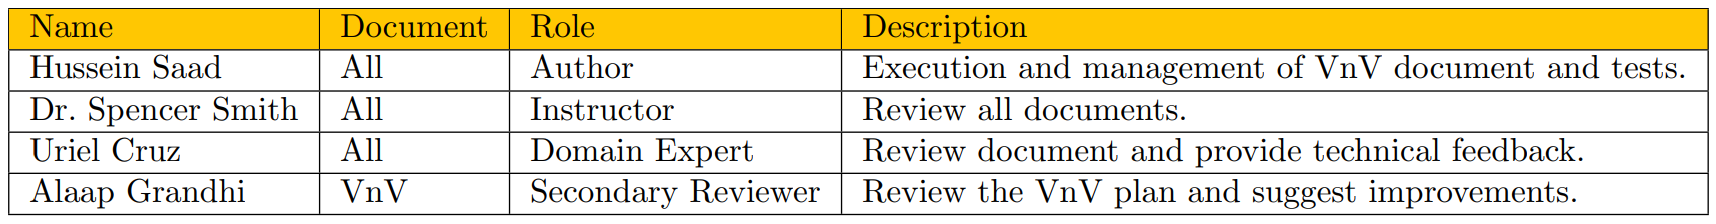
\includegraphics[scale=0.35]{VnVTeam.PNG} \label{team_table}
  \captionof{table}{Verification Team}
\end{center}

\subsection{SRS Verification Plan}
The Optimal EM Placement SRS document will be verified solely through ad hoc feedback from reviewers. Document design and alignment with course goals will be reviewed by the instructor (Dr.~Spencer Smith), while more technical details will benefit from the comments of the Domain Expert Reviewer (Uriel Cruz). After the creation/update of the SRS document, reviewers will provide the author with feedback through GitHub issues. The author will implement the suggested changes as necessary.

\subsection{Design Verification Plan}
The design documents, Module Guide (MG) and Module Interface Specification (MIS), will be verified through inspection by reviewers. 

\subsection{Verification and Validation Plan Verification Plan}
The Verification and Validation Plan will itself be verified primarily through manual reviews by the Instructor, Domain Expert, and Secondary Reviewer.

\subsection{Implementation Verification Plan}
The implementation of Optimal EM Placement will be verified primarily in two different ways:
\begin{enumerate}
  \item \textbf{Code Walkthrough (Static): }Walkthroughs will be performed by the author, domain expert, and secondary reviewer. Copies of the code will be shared with all three team members, who will individually run and interact with the program. This process is followed by a discussion in which members discuss their findings and suggest enhancements. 
  \item \textbf{Test Cases (Dynamic): }As outlined in Section \ref{sys_tests}, test cases will be executed to verify the function and non-functional requirements mentioned in the SRS. 
\end{enumerate}

\subsection{Automated Testing and Verification Tools} \label{ver_tools}
Automated testing as outlined in the previous section will be carried out using the \href{https://docs.pytest.org/en/stable/}{\texttt{PyTest}} library, by comparing expected outputs to calculated outputs given some constant user input. 

\section{System Tests} \label{sys_tests}

\subsection{Tests for Functional Requirements}
The functional and nonfunctional requirements of the program are given in Sections 5.1 and 5.2 of the \href{https://github.com/husseinsd1/optimal-em-arrangement/blob/main/docs/SRS/SRS.pdf}{SRS}. The relationship between test cases and requirements is given in the traceability matrix in Section \ref{trac_matrix}. \\ \\
\noindent \emph{Error codes in Table \ref{emprop} are explained in Section \ref{abbrevs} of the document.}


\subsubsection{Input Tests - Invalid Input}

		
\paragraph{Incorrect EM Properties}
\begin{center}
  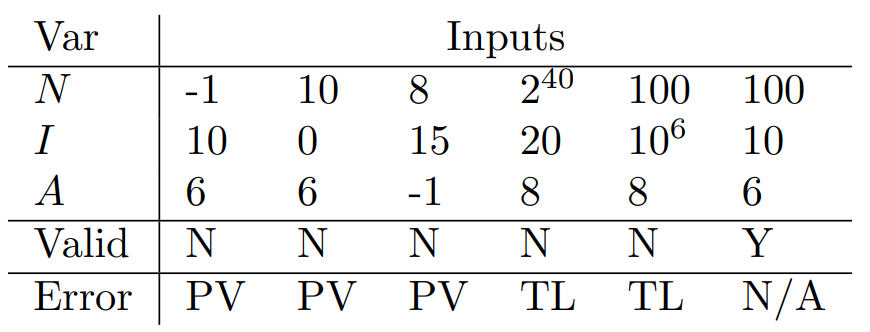
\includegraphics[scale=0.4]{EMInputTable.PNG} \\
  \captionof{table}{EM properties test cases}
  \label{emprop}
\end{center}

\begin{enumerate}

\item{test-em-props-1\dots6\\}

Control: Automatic.
					
Initial State: Pending input.
					
Input: Set of input values for EM Properties as given in Table \ref{emprop}.
					
Output: An appropriate error message, if necessary, as given in Table \ref{emprop}.

Test Case Derivation: These cases test the behaviour of the system when given invalid system related inputs as described in Table 2 of the SRS.
					
How test will be performed: Using \texttt{PyTest}. 
\end{enumerate}

\newpage

\paragraph{System Setup}
\begin{center}
  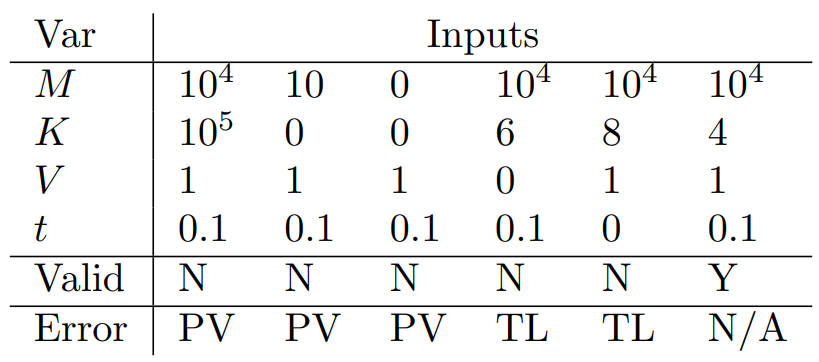
\includegraphics[scale=0.4]{SysInputTable.PNG} \\
  \captionof{table}{System setup test cases}
  \label{sys_setup_table}
\end{center}

\begin{enumerate}

  \item{test-sys-setup-1\dots6\\}
  
  Control: Automatic.
            
  Initial State: Pending input.
            
  Input: Set of input values for the system as given in Table \ref{sys_setup_table}.
            
  Output: An appropriate error message, if necessary, as given in Table~\ref{sys_setup_table}.
  
  Test Case Derivation: These cases test the behaviour of the system when given invalid EM related inputs as described in Table 2 of the SRS.
            
  How test will be performed: Using \texttt{PyTest}. 
\end{enumerate}

\subsubsection{Output Tests - Correct Output}
\paragraph{Correct Positions Selected}
\begin{center}
  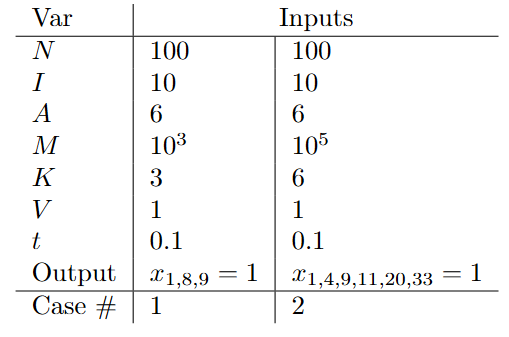
\includegraphics[scale=0.4]{OutputTable.PNG} \\
  \captionof{table}{Output correctness test cases}
  \label{output_tests_table}
\end{center}

\begin{enumerate}

  \item{test-output-correct-1\dots2\\}
  
  Control: Automatic.
            
  Initial State: Pending input.
            
  Input: Set of input values for as given in Table~\ref{output_tests_table}.
            
  Output: A binary vector $x$, such that the indices shown in Table~\ref{output_tests_table} are 1.

  Note: The above must hold for a set \texttt{numpy} random seed of 100. 
  
  Test Case Derivation: These cases ensure the system returns the correct optimal positions based on the inputs it receives. 
            
  How test will be performed: Using \texttt{PyTest}. 
\end{enumerate}

\subsubsection{Intermediate Tests - Intermediate Computations} \label{svd_test}
\paragraph{Singular Values}

\begin{enumerate}

  \item{test-intmed-svd-1\dots2\\} 
  
  Control: Automatic.
            
  Initial State: Pending input.
            
  Input: Set of input values for as given in Table \ref{output_tests_table}.
            
  Output: An array of singular values. 
  
  Test Case Derivation: These cases ensure the program is correctly constructing the $\mathcal{U}$ matrix and computing the magnetic field and force values. A description of $\mathcal{U}$ is given in Section 4.2.4 of the SRS.
            
  How test will be performed: Using \texttt{PyTest}. 
\end{enumerate}

\subsection{Tests for Nonfunctional Requirements}
The 4 nonfunctional requirements for Optimal EM placement is given in Section 5.2 of the SRS. 
\subsubsection{Accuracy}
\begin{enumerate}

\item{test-nf-acc\\}

Type: Manual.
					
Initial State: Pending input.
					
Input: Any set of inputs as given in Table \ref{output_tests_table}.
					
Output: The singular values of the $\mathcal{U}$.
					
How test will be performed: The author will use identical inputs on naïve algorithms and plot a singular value distribution to compare performance, as explained in NF1 of the SRS. This test related to the Singular Values test in \ref{svd_test}.
\end{enumerate}

\subsubsection{Usability}
\begin{enumerate}

\item{test-nf-use\\}

Type: Manual.
					
Initial State: None.
					
Input: None.
					
Output: None.
					
How test will be performed: A group of users will be asked to use the system and attempt to get a solution for their inputs. They will then provide any necessary feedback. 
\end{enumerate}

\subsubsection{Maintainability}
\begin{enumerate}

\item{test-nf-mtn\\}

Type: Static.
					
Initial State: None.
					
Input: None.
					
Output: None.
					
How test will be performed: The author will meet with the Domain Expert Reviewer and Secondary Reviewer to present a code walkthrough and discuss details related to software maintainability. 
\end{enumerate}

\subsubsection{Portability}
\begin{enumerate}

\item{test-nf-prt\\}

Type: Manual.
					
Initial State: None.
					
Input: None.
					
Output: None.
					
How test will be performed: The author will run the program on a Windows, MacOS and Linux machine. 
\end{enumerate}

\subsection{Traceability Between Test Cases and Requirements} \label{trac_matrix}
Traceability between tests and requirements is visualized below:
\begin{center}
  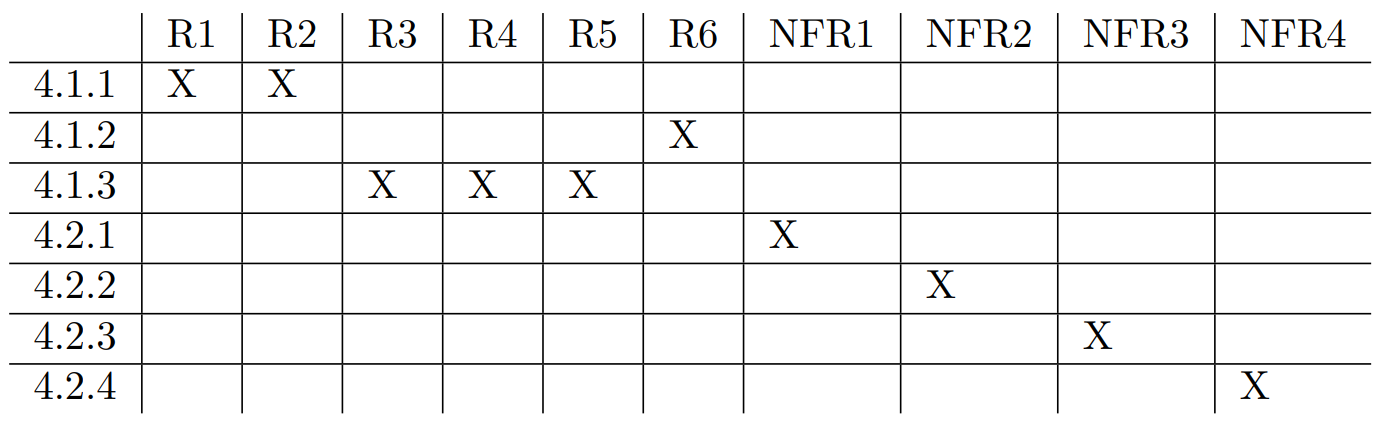
\includegraphics[scale=0.4]{TraceabilityMatrix.PNG}
  \captionof{table}{Traceability between tests and requirements}
\end{center}




%%%%%%%%%%%%%%%%%%%%%%%%%%%%%%%%%%%%%%%%%%%%






\newpage
\section{Unit Test Description} \label{unit_tests}

\wss{This section should not be filled in until after the MIS (detailed design
  document) has been completed.}

\wss{Reference your MIS (detailed design document) and explain your overall
philosophy for test case selection.}  

\wss{To save space and time, it may be an option to provide less detail in this section.  
For the unit tests you can potentially layout your testing strategy here.  That is, you 
can explain how tests will be selected for each module.  For instance, your test building 
approach could be test cases for each access program, including one test for normal behaviour 
and as many tests as needed for edge cases.  Rather than create the details of the input 
and output here, you could point to the unit testing code.  For this to work, you code 
needs to be well-documented, with meaningful names for all of the tests.}

\subsection{Unit Testing Scope}

\wss{What modules are outside of the scope.  If there are modules that are
  developed by someone else, then you would say here if you aren't planning on
  verifying them.  There may also be modules that are part of your software, but
  have a lower priority for verification than others.  If this is the case,
  explain your rationale for the ranking of module importance.}

\subsection{Tests for Functional Requirements}

\wss{Most of the verification will be through automated unit testing.  If
  appropriate specific modules can be verified by a non-testing based
  technique.  That can also be documented in this section.}

\subsubsection{Module 1}

\wss{Include a blurb here to explain why the subsections below cover the module.
  References to the MIS would be good.  You will want tests from a black box
  perspective and from a white box perspective.  Explain to the reader how the
  tests were selected.}

\begin{enumerate}

\item{test-id1\\}

Type: \wss{Functional, Dynamic, Manual, Automatic, Static etc. Most will
  be automatic}
					
Initial State: 
					
Input: 
					
Output: \wss{The expected result for the given inputs}

Test Case Derivation: \wss{Justify the expected value given in the Output field}

How test will be performed: 
					
\item{test-id2\\}

Type: \wss{Functional, Dynamic, Manual, Automatic, Static etc. Most will
  be automatic}
					
Initial State: 
					
Input: 
					
Output: \wss{The expected result for the given inputs}

Test Case Derivation: \wss{Justify the expected value given in the Output field}

How test will be performed: 

\item{...\\}
    
\end{enumerate}

\subsubsection{Module 2}

...

\subsection{Tests for Nonfunctional Requirements}

\wss{If there is a module that needs to be independently assessed for
  performance, those test cases can go here.  In some projects, planning for
  nonfunctional tests of units will not be that relevant.}

\wss{These tests may involve collecting performance data from previously
  mentioned functional tests.}

\subsubsection{Module ?}
		
\begin{enumerate}

\item{test-id1\\}

Type: \wss{Functional, Dynamic, Manual, Automatic, Static etc. Most will
  be automatic}
					
Initial State: 
					
Input/Condition: 
					
Output/Result: 
					
How test will be performed: 
					
\item{test-id2\\}

Type: Functional, Dynamic, Manual, Static etc.
					
Initial State: 
					
Input: 
					
Output: 
					
How test will be performed: 

\end{enumerate}

\subsubsection{Module ?}

...

\subsection{Traceability Between Test Cases and Modules}

\wss{Provide evidence that all of the modules have been considered.}

\newpage

\bibliographystyle{plainnat}

\bibliography{../../refs/References}

\newpage

\section{Appendix}

This is where you can place additional information.

\subsection{Symbolic Parameters}

The definition of the test cases will call for SYMBOLIC\_CONSTANTS.
Their values are defined in this section for easy maintenance.

\subsection{Usability Survey Questions?}

\wss{This is a section that would be appropriate for some projects.}

\end{document}